%o que são redes neurais
Redes Neurais Artificiais (RNAs) são modelos computacionais bioinspirados no sistema neurológico humano. A motivação para o desenvolvimento e uso destes modelos é a grande complexidade do cérebro humano, definido por \citeonline{Haykin1998} como um computador altamente complexo, não linear e paralelo. O autor ainda define uma RNA como``\textit{a machine that is designed to} model \textit{the way in which the brain performs a particular task or function of interest}''\footnote{``uma máquina que é desenvolvida para \textit{modelar} a forma como o cérebro desempenha uma tarefa específica ou função de interesse'' (tradução nossa).}. Seguindo o modelo biológico do cérebro humano, uma RNA é composta por neurônios artificiais e pelas interações existentes entre estes neurônios: as sinapses.

%Explicação simplificada do sistema nervoso
A \autoref{fig:brainsistem} ilustra, em um diagrama de blocos, o sistema nervoso como um sistema de três estágios. A Rede Neural representa o cérebro em si, que recebe informações continuamente, as percebe e toma as decisões apropriadas para cada uma delas \cite[p.~24]{Haykin1998}.

\begin{figure}[!htb]
    \centering
    \caption{Representação em digrama de blocos do sistema nervoso}
    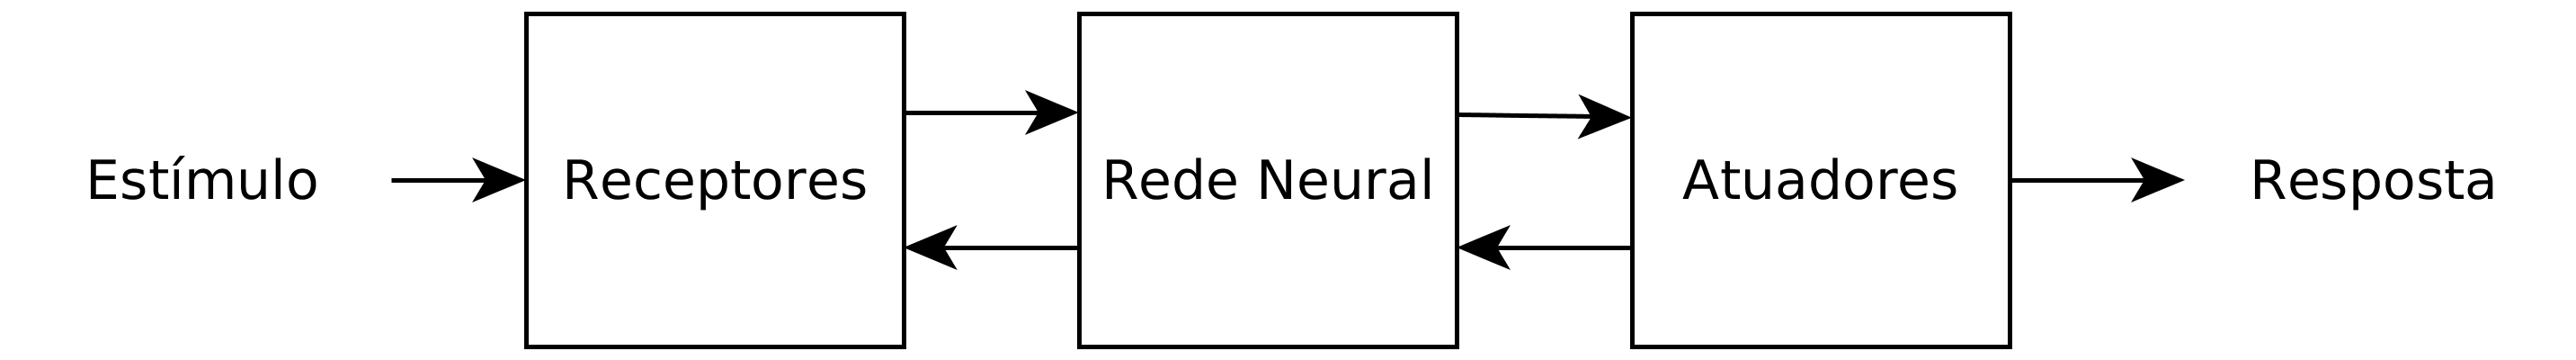
\includegraphics[width=0.9\textwidth]{./04-figuras/brain_sistem_block_diagram}
    \fonte{Adaptado de \citeonline[p.~28]{Haykin1998}}
    \label{fig:brainsistem}
\end{figure}

%O que são sinapses
Toda esta comunicação se dá a partir de sinapses, que são unidades estruturais e funcionais que mediam a interação entre neurônios. Seu funcionamento simplificado é o seguinte: o processo pré-sináptico libera uma substância transmissora que é difundida através da junção sináptica entre neurônios e então age sobre o processo pós-sináptico. Então, a sinapse converte o sinal elétrico pré-sinápitico em um sinal químico e, por fim, de volta a um sinal elétrico pós-sináptico \cite[p.~28]{Haykin1998}. É por meio deste processo de comunicação entre neurônios que adquirimos novos conhecimentos e relacionamos estímulos a respostas. É também devido a ele que podemos fazer associações diversas com acontecimentos no passado, evento que chamamos de \textit{memória}. O imenso poder que os neurônios possuem inspirou modelagens computacionais capazes de atuar em situações em que se deseja obter respostas adequadas a diferentes estímulos, e em outras relacionadas à memória e aprendizado. Um modelo neural comumente aplicado na literatura em problemas relacionados às RNAs é o perceptron. 

Um perceptron é um modelo computacional de um neurônio não linear e é ilustrado na Figura \ref{fig:neuronmodel}, em que $y_k$ é a saída do sistema obtido após o processamento neural relacionado às entradas $x_i$, cada qual contribuindo com um peso $w_{ki}$ para a junção de soma representada pelo bloco $\sum$. O processamento neural envolve ainda a função de ativação $\phi$ que, de acordo com o valor obtido na junção de soma, define o valor da saída $y_k$. Se o valor $v_k$ for maior que um limiar pré-determinado, a saída do sistema é ativada e terá o valor 1, caso contrário assumirá o valor 0, simulando assim o processo de transmissão ou não de impulsos elétricos que ocorrem nos neurônios biológicos.

\begin{figure}[!htb]
    \centering
    \caption{Modelo não linear de um neurônio}
    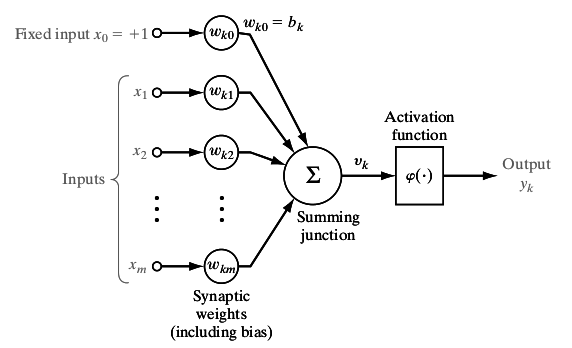
\includegraphics[width=0.9\textwidth]{./04-figuras/neuron-diagram-gray}
    \fonte{Adaptado de \citeonline[p.~33]{Haykin1998}}
    \label{fig:neuronmodel}
\end{figure}

O modelo simples de um neurônio representado por perceptrons permite a simulação das já definidas sinapses, possibilitando a criação de RNAs complexas formadas por múltiplos neurônios, organizados em cadeias, como é mostrado na Figura \ref{fig:rna}. Neste exemplo, $x_1$, $x_2$ e $x_3$ são as entradas do sistema; os blocos 4, 5 e 6 representam, cada qual, um neurônio numa camada escondida; os blocos 7 e 8 representam os dois neurônios que compõem a camada de saída; e, por fim, $x_7$ e $x_8$ são as saídas de RNA. Redes como essa, que possuem mais de uma camada de neurônios, são denominadas \textit{Multilayer Perceptron} (MLP\footnote{Perceptron Multicamada (tradução nossa).}). As diferentes combinações que se podem obter distribuindo os neurônios de uma RNA de diferentes maneiras fazem com que estas redes possam ser utilizadas em aplicações diversas relacionadas à IA e IC.



\begin{figure}[!htb]
    \centering
    \caption{Modelo de um \textit{MLP}}
    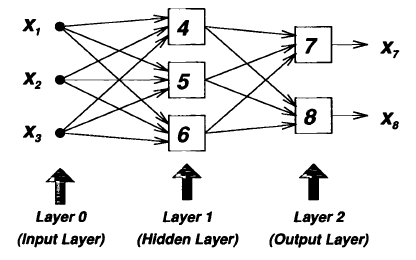
\includegraphics[width=0.6\textwidth]{./04-figuras/fund_teorica/rna}
    \fonte{\citeonline[p.~205]{Jang1997}}
    \label{fig:rna}
\end{figure}

%vantagens das RNAs/ Funcionamento das RNAs
A principal característica de uma rede neural artificial que a torna interessante para aplicações computacionais é a sua capacidade de aprendizado. O procedimento usado para efetuar o processo de aprendizado é chamado \textit{algoritmo de aprendizado}, cuja função é modificar os pesos sinápticos da rede de forma ordenada para atingir um objetivo desejado \cite[p.~24]{Haykin1998}. É a partir deste aprendizado que as RNAs alcançam uma ótima taxa de generalização, fazendo delas fortes aliadas, por exemplo, para reconhecimento de padrões. Controladores que utilizam técnicas relacionadas a RNAs se beneficiam justamente destas capacidades de aprendizado e generalização conferidas por elas.

O controlador desenvolvido neste trabalho utiliza RNAs com treinamento supervisionado, que são treinadas a partir de um conjunto de entradas mapeadas no valor de suas respectivas saídas, resultando na obtenção de um conjunto de retas com parâmetros ajustados de acordo com os dados do treinamento. São as retas obtidas após este treinamento que conferem à rede o poder de generalização, permitindo que novas entradas sejam mapeadas para saídas que condizem com o cenário em questão.

Além disto, como o controlador projetado é do tipo Neuro-\textit{Fuzzy}, as retas ajustadas após o treinamento se enquadram num grupo especial correspondendo cada qual a uma função de pertinência de conjuntos \textit{Fuzzy}, assunto este que é abordado na seção seguinte.
